% https://github.com/martinhelso/UiB

\documentclass[UKenglish]{beamer}

\usetheme{UiB}

\usepackage[utf8]{inputenx} % For æ, ø, å
\usepackage{csquotes}	    % Quotation marks
\usepackage{microtype}	    % Improved typography
\usepackage{amssymb}	    % Mathematical symbols
\usepackage{mathtools}	    % Mathematical symbols
\usepackage[absolute, overlay]{textpos} % Arbitrary placement
\setlength{\TPHorizModule}{\paperwidth} % Textpos units
\setlength{\TPVertModule}{\paperheight} % Textpos units
\usepackage{tikz}
\usepackage{pgfplots}
\usepackage{minted}
\usepackage{xcolor}
\usepackage{tabto}
\usepackage{amsmath}
\setminted{xleftmargin=1cm}
\usetikzlibrary{overlay-beamer-styles}	% Overlay effects for TikZ
\usefonttheme[onlymath]{serif}

\usepackage{verbatim}

\author{Kenneth Langedal}
\title{Matrix Multiplication}
\subtitle{Demystifying the Inner Workings of BLAS Libraries}

\begin{document}

\setbeamertemplate{caption}{\raggedright\insertcaption\par}

\begin{frame}[c]{The Problem}

    \begin{center}
        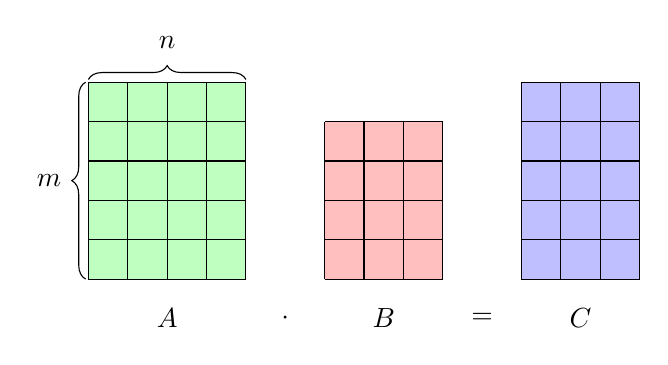
\begin{tikzpicture}
            \draw (1,-0.5) node{$A$};
            \fill[green, opacity=0.25] (0,0) rectangle ++(2,2.5);
            \draw[step=0.5cm,black] (0,0) grid ++(2,2.5);

            \draw (2.5,-0.5) node{$\cdot$};

            \draw (3.75,-0.5) node{$B$};
            \fill[red, opacity=0.25] (3,0) rectangle ++(1.5,2);
            \draw[step=0.5cm,black] (3-0.001,0-0.001) grid
            ++(1.5+0.001,2+0.001);

            \draw (5,-0.5) node{$=$};

            \draw (6.25,-0.5) node{$C$};
            \fill[blue, opacity=0.25] (5.5,0) rectangle ++(1.5,2.5);
            \draw[step=0.5cm,black] (5.5-0.001,0-0.001) grid
            ++(1.5+0.001,2.5+0.001);

            \uncover<2>{\draw [decorate,decoration={brace, amplitude=5pt,
                            raise=1pt}] (0,0) -- (0,2.5) node[midway, xshift=-0.5cm]{$m$};}

            \uncover<2>{\draw [decorate,decoration={brace, amplitude=5pt,
                            raise=1pt}] (0,2.5) -- (2,2.5) node[midway, yshift=0.5cm]{$n$};}

        \end{tikzpicture}
    \end{center}
\end{frame}

\begin{frame}[c, noframenumbering]{The Problem}
    \begin{center}
        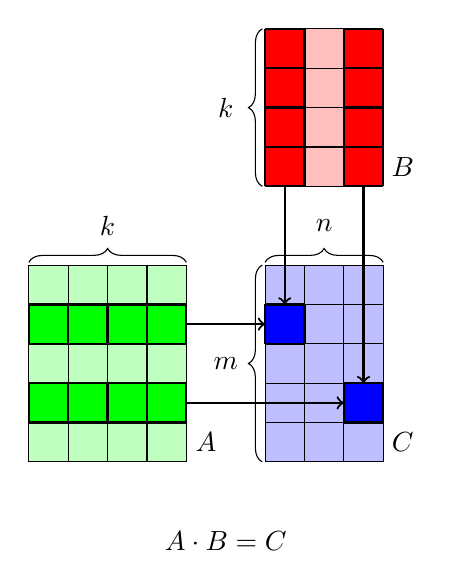
\begin{tikzpicture}
            \draw (2.5,-1) node{$A \cdot B = C$};

            \draw (2.25,0.25) node{$A$};
            \fill[green, opacity=0.25] (0,0) rectangle ++(2,2.5);
            \draw[step=0.5cm,black] (0,0) grid ++(2,2.5);

            \draw (4.75,0.25) node{$C$};
            \fill[blue, opacity=0.25] (3,0) rectangle ++(1.5,2.5);
            \draw[step=0.5cm,black] (3-0.001,0-0.001) grid
            ++(1.5+0.001,2.5+0.001);

            \draw (4.75,3.75) node{$B$};
            \fill[red, opacity=0.25] (3,3.5) rectangle ++(1.5,2);
            \draw[step=0.5cm,black] (3-0.001,3.5-0.001) grid
            ++(1.5+0.001,2+0.001);

            \uncover<2-3>{
                \draw [decorate,decoration={brace, amplitude=5pt, raise=1pt}]
                (3,3.5) -- (3,5.5) node[midway, xshift=-0.5cm]{$k$};
                \draw [decorate,decoration={brace, amplitude=5pt, raise=1pt}]
                (0,2.5) -- (2,2.5) node[midway, yshift=0.5cm]{$k$};
            }

            \uncover<3>{
                \draw [decorate,decoration={brace, amplitude=5pt, raise=1pt}]
                (3,0) -- (3,2.5) node[midway, xshift=-0.5cm]{$m$};
                \draw [decorate,decoration={brace, amplitude=5pt, raise=1pt}]
                (3,2.5) -- (4.5,2.5) node[midway, yshift=0.5cm]{$n$};
            }

            \uncover<4>{
                \draw[->, thick] (2,1.75) -- (3,1.75);
                \draw[->, thick] (3.25,3.5) -- (3.25,2);
                \fill[green] (0,2) rectangle (2,1.5);
                \draw[step=0.5cm,black,thick] (0-0.001,2+0.001) grid
                (2+0.001,1.5-0.001);
                \fill[red] (3,5.5) rectangle (3.5,3.5);
                \draw[step=0.5cm,black,thick] (3-0.001,5.5+0.001) grid
                (3.5+0.001,3.5-0.001);
                \fill[blue] (3,2) rectangle (3.5,1.5);
                \draw[step=0.5cm,black,thick] (3-0.001,2+0.001) grid
                (3.5+0.001,1.5-0.001);
            }
            \uncover<5>{
                \draw[->, thick] (2,0.75) -- (4,0.75);
                \draw[->, thick] (4.25,3.5) -- (4.25,1);
                \fill[green] (0,1) rectangle (2,0.5);
                \draw[step=0.5cm,black,thick] (0-0.001,1+0.001) grid
                (2+0.001,0.5-0.001);
                \fill[red] (4,5.5) rectangle (4.5,3.5);
                \draw[step=0.5cm,black,thick] (4-0.001,5.5+0.001) grid
                (4.5+0.001,3.5-0.001);
                \fill[blue] (4,1) rectangle (4.5,0.5);
                \draw[step=0.5cm,black,thick] (4-0.001,1+0.001) grid
                (4.5+0.001,0.5-0.001);
            }

        \end{tikzpicture}
    \end{center}
\end{frame}

\begin{frame}[fragile,c]{First Naive Implementation}
    \begin{exampleblock}{Python, naive}
        \begin{minted}[
fontsize=\footnotesize,
linenos
]{python}
for i in range(M):
    for j in range(N):
        for k in range(K):
            C[i][j] += A[i][k] * B[k][j]
\end{minted}
    \end{exampleblock}
    \pause
    \begin{itemize}
        \item For $M=N=K=512$, this code takes 61 seconds
              \pause
        \item OpenBLAS computes the same in 0.0048 seconds
              \pause
        \item More than 12000 times faster
    \end{itemize}
    \pause
    \begin{columns}
        \begin{column}{0.75\textwidth}
            \begin{alertblock}{Python, NumPy}
                \begin{minted}[
fontsize=\footnotesize,
linenos
]{python}
import numpy as np
C = np.matmul(A, B)
\end{minted}
            \end{alertblock}
        \end{column}
    \end{columns}
\end{frame}

\begin{frame}[c]{First Naive Implementation}
    \begin{itemize}
        \item Python using CPython \tab $\Longrightarrow$ 61 seconds
              \pause
        \item Python using PyPy 3 \tab $\Longrightarrow$ 2 seconds
              \pause
        \item C using GCC 11.4 (-O3) \tab $\Longrightarrow$ 0.54 seconds
              \pause
        \item OpenBLAS \tab $\Longrightarrow$ 0.0048 seconds
    \end{itemize}

    \pause
    \begin{alertblock}{NumPy to C}
        \small
        Naive implementation in C is more than 100 times slower than OpenBLAS
    \end{alertblock}
\end{frame}

\begin{frame}[c]{Performance Progression}

    \begin{figure}
        \centering
        \begin{tikzpicture}
            \begin{axis}[
                    width=0.9\textwidth,
                    height=0.8\textheight,
                    symbolic x coords={CPython,PyPy 3,C},
                    xtick=data,
                    axis x line=center,
                    axis y line=left,
                    enlargelimits=true,
                    enlarge x limits=0.25,
                    ylabel={GFLOPS ($\frac{M*N*K*2}{time (s)}$)},
                    nodes near coords,
                    nodes near coords style={font=\tiny},
                    every axis plot/.append style={
                            ybar,
                            bar width=20,
                            bar shift=0pt,
                            fill
                        }]
                \addplot[ybar,fill=blue,width=10] coordinates {
                        (CPython,0.004)
                        (PyPy 3,0.13)
                        (C,0.49)
                    };
            \end{axis}
        \end{tikzpicture}
        \caption{i7-9750H CPU locked at 2 GHz using single precision floats}
        \label{fig:enter-label}
    \end{figure}
\end{frame}

\begin{frame}[c, noframenumbering]{Performance Progression}

    \begin{figure}
        \centering
        \begin{tikzpicture}
            \begin{axis}[
                    width=0.9\textwidth,
                    height=0.8\textheight,
                    symbolic x coords={CPython,PyPy 3,C,OpenBLAS},
                    xtick=data,
                    axis x line=center,
                    axis y line=left,
                    ytick={0,16,32,48,64},
                    ymax=64,
                    ymin=0,
                    enlargelimits=true,
                    enlarge x limits=0.25,
                    ylabel={GFLOPS ($\frac{M*N*K*2}{time (s)}$)},
                    nodes near coords,
                    nodes near coords style={font=\tiny},
                    every axis plot/.append style={
                            ybar,
                            bar width=20,
                            bar shift=0pt,
                            fill
                        }]
                \addplot[ybar,fill=blue,width=10] coordinates {
                        (CPython,0.004)
                        (PyPy 3,0.13)
                        (C,0.49)
                        (OpenBLAS, 60.25)
                    };
                \draw[dashed] (axis cs:CPython,64) -- node[above,font=\small]{Theoretical
                    Limit} ++(250,0);
            \end{axis}
        \end{tikzpicture}
        \caption{i7-9750H CPU locked at 2 GHz using single precision floats}
        \label{fig:enter-label}
    \end{figure}
\end{frame}

\section{Theoretical Background}
%\SectionPage

\begin{frame}[c]{Algorithms}
    \small
    \begin{itemize}
        \pause
        \item Assume $n=m=k$
              \pause
        \item Naive algorithm \tab $\Longrightarrow \mathcal{O}(n^3)$
              \pause
        \item Strassen’s algorithm 1969 \tab $\Longrightarrow
                  \mathcal{O}(n^{2.8074})$
              \pause
        \item \dots
        \item Williams, Xu, Xu, and Zhou 2023 \tab $\Longrightarrow
                  \mathcal{O}(n^{2.3716})$
    \end{itemize}
\end{frame}

\begin{comment}
\begin{frame}[c]{Algorithms}
    \begin{figure}
        \centering
        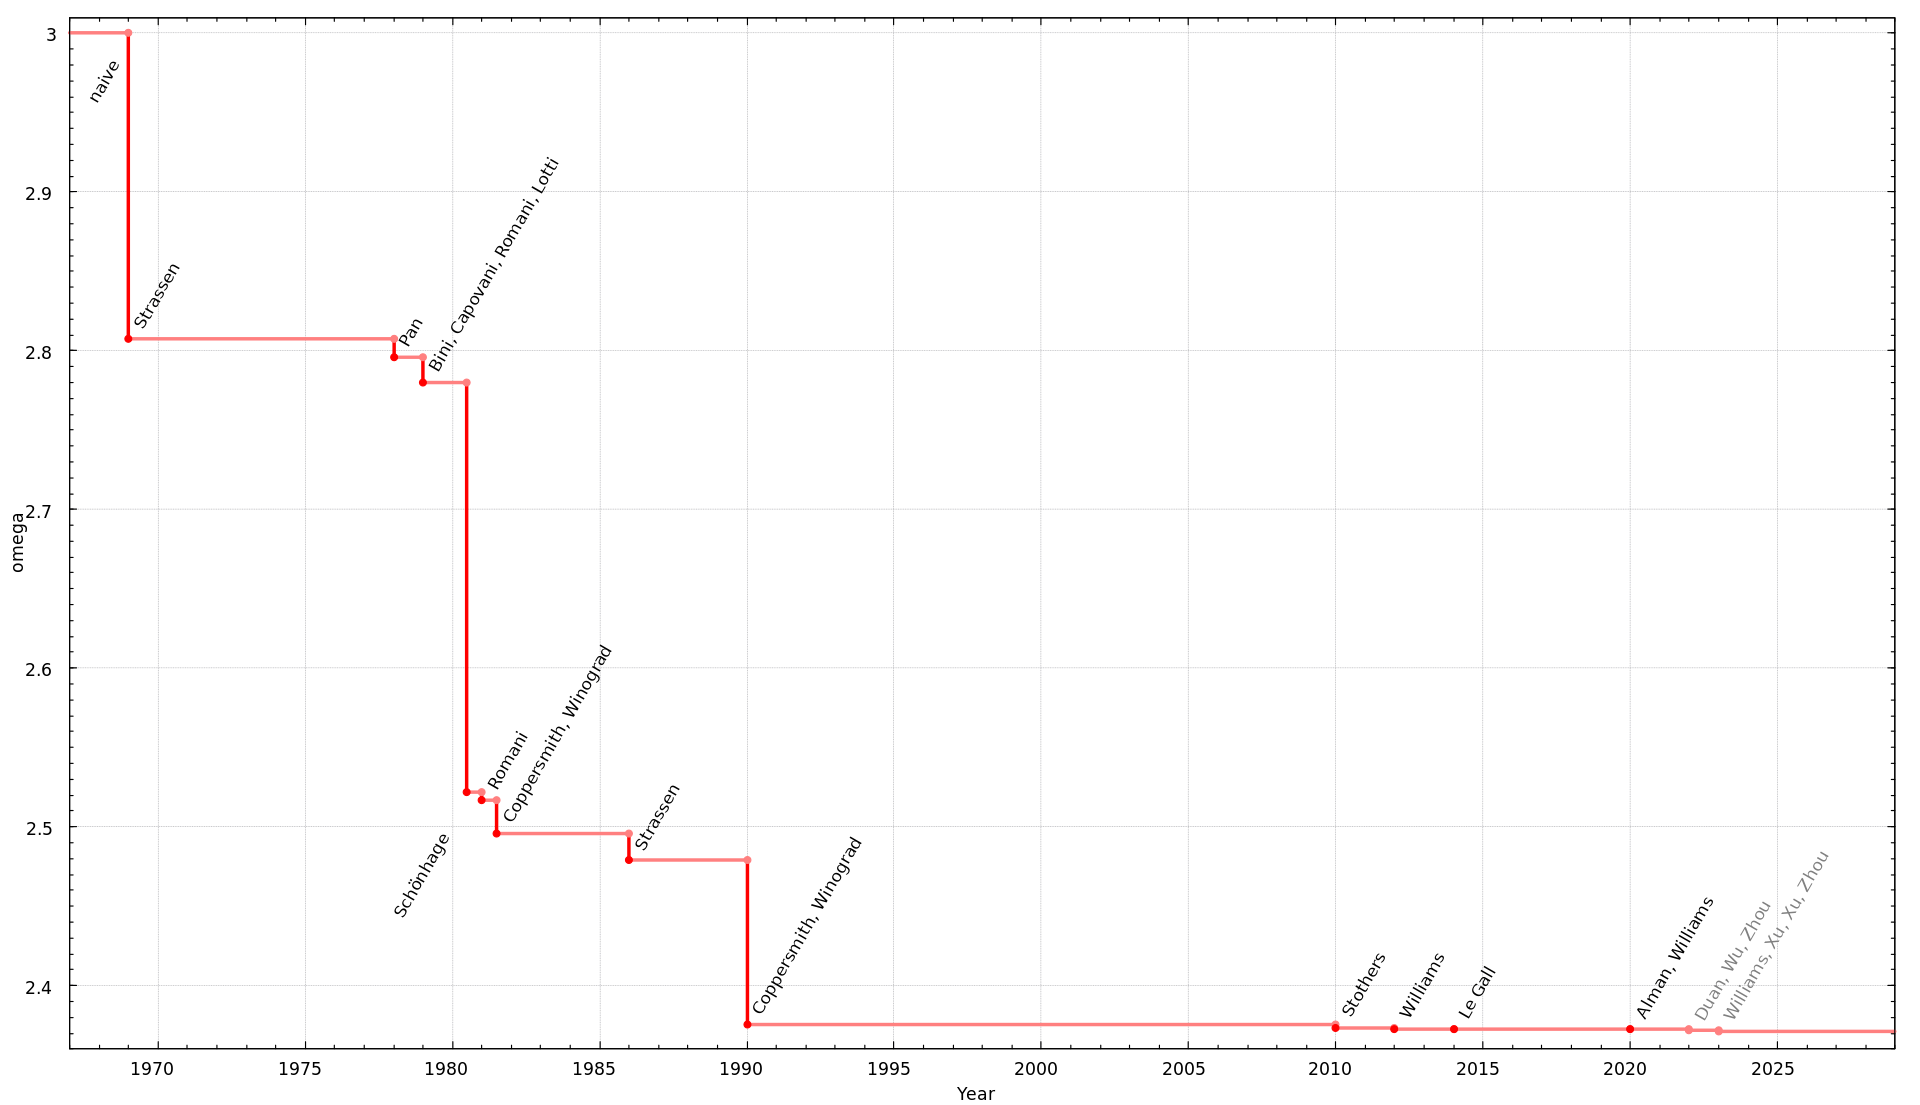
\includegraphics[scale=0.15]{data/MatrixMultComplexity_svg.svg.png}
        \caption{}
    \end{figure}
\end{frame}
\end{comment}

\begin{frame}[c]{Why don't we use Strassen's algorithm?}
    \begin{itemize}
        \pause
        \item Bjørstad, Manne, Sørevik, and Vajteršic 1992 \break \alert{50\%
                  faster at $N = 2048$}
              \pause
        \item Douglas, Heroux, Slishman, and Smith 1993 \break \alert{10-40\%
                  faster at $N = 1826$}
              \pause
        \item Huss-Lederman, Jacobson, Tsao, Turnbull, and Johnson 1996 \break
              \alert{10-20\% faster than Douglas et al.}
              \pause
        \item D'alberto, Bodrato, and Nicolau 2011 \break \alert{5–25\% faster
                  $N = 6500$}
              \pause
        \item Huang, Smith, Henry, and Van De Geijn 2016 \break \alert{20\%
                  faster $N = 16000$}
              \pause
        \item Comes at the cost of numerical stability and additional memory
        \item Needs large $N$ to really outperform the naive algorithm
    \end{itemize}
\end{frame}

\begin{frame}[c]{Strassen’s Algorithm}
    \begin{center}
        $A=
            \begin{pmatrix}
                A_{11} & A_{12} \\
                A_{21} & A_{22}
            \end{pmatrix}
            \quad
            B=
            \begin{pmatrix}
                B_{11} & B_{12} \\
                B_{21} & B_{22}
            \end{pmatrix}
            \quad
            A \cdot B =
            \begin{pmatrix}
                C_{11} & C_{12} \\
                C_{21} & C_{22}
            \end{pmatrix}
        $
    \end{center}
    \pause
    \footnotesize
    \begin{columns}[onlytextwidth]
        \begin{column}{0.49\textwidth}
            \begin{align*}
                \mathrm{I}   & = (A_{11}+A_{22})(B_{11}+B_{22})  \\
                \mathrm{II}  & = (A_{21}+A_{22})B_{11}           \\
                \mathrm{III} & = A_{11}(B_{12}-B_{22})           \\
                \mathrm{IV}  & = A_{22}(-B_{11}+B_{21})          \\
                \mathrm{V}   & = (A_{11}+A_{12})B_{22}           \\
                \mathrm{VI}  & = (-A_{11}+A_{21})(B_{11}+B_{12}) \\
                \mathrm{VII} & = (A_{12}-A_{22})(B_{21}+B_{22})  \\
            \end{align*}
        \end{column}
        \begin{column}{0.49\textwidth}
            \vfill
            \begin{align*}
                C_{11} & = \mathrm{I} + \mathrm{IV} - \mathrm{V} + \mathrm{VII}  \\
                C_{12} & = \mathrm{III} + \mathrm{V}                             \\
                C_{21} & = \mathrm{II} + \mathrm{IV}                             \\
                C_{22} & = \mathrm{I} + \mathrm{III} - \mathrm{II} + \mathrm{VI}
            \end{align*}
        \end{column}
    \end{columns}
    \pause
    \begin{center}
        $T(n)=7T(\frac{n}{2})+\mathcal{O}(n^2)$ \\ \vfill
        \pause
        $\mathcal{O}(n^{\text{log}_2 7}) \approx \mathcal{O}(n^{2.81})$
    \end{center}
\end{frame}

\section{Bridging the gap to ObenBLAS}
%\SectionPage

\begin{frame}[c]{Memory Layout}
    \begin{itemize}
        \item Matrices are stored in row-major order
    \end{itemize}
    \vfill
    \begin{center}
        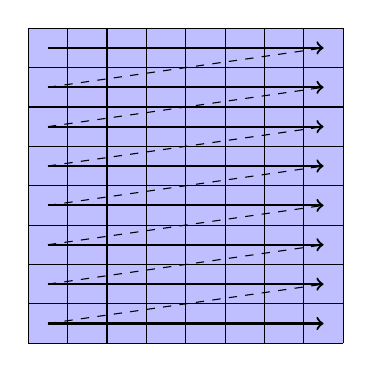
\begin{tikzpicture}
            \fill[blue, opacity=0.25] (0,0) rectangle ++(4,4);
            \draw[step=0.5cm,black] (0-0.001,0-0.001) grid ++(4+0.001,4+0.001);

            \uncover<2>{
                \foreach \i in {0.25,0.75,...,3.25} {
                        \draw[->, thick] (0.25,\i) -- (3.75,\i);
                        \draw[-, dashed] (0.25,\i) -- (3.75,\i + 0.5);
                    }
                \draw[->, thick] (0.25,3.75) -- (3.75,3.75);
            }
        \end{tikzpicture}
    \end{center}
\end{frame}

\begin{frame}[c, noframenumbering]{Memory Layout}
    \begin{center}
        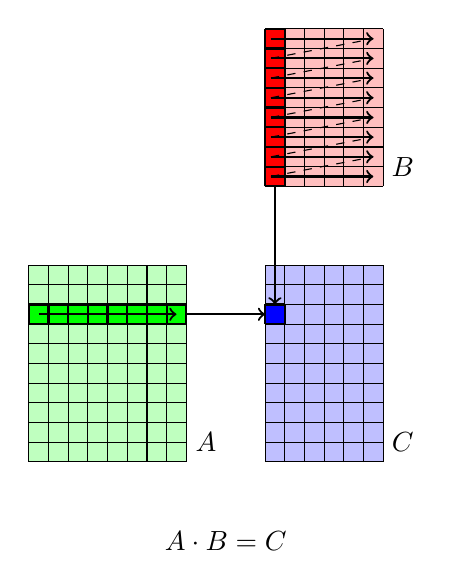
\begin{tikzpicture}
            \draw (2.5,-1) node{$A \cdot B = C$};

            \draw (2.25,0.25) node{$A$};
            \fill[green, opacity=0.25] (0,0) rectangle ++(2,2.5);
            \draw[step=0.25cm,black] (0,0) grid ++(2,2.5);

            \draw (4.75,0.25) node{$C$};
            \fill[blue, opacity=0.25] (3,0) rectangle ++(1.5,2.5);
            \draw[step=0.25cm,black] (3-0.001,0-0.001) grid
            ++(1.5+0.001,2.5+0.001);

            \draw (4.75,3.75) node{$B$};
            \fill[red, opacity=0.25] (3,3.5) rectangle ++(1.5,2);
            \draw[step=0.25cm,black] (3-0.001,3.5-0.001) grid
            ++(1.5+0.001,2+0.001);

            \uncover<2-3>{
                \draw[->, thick] (2,1.875) -- (3,1.875);
                \draw[->, thick] (3.125,3.5) -- (3.125,2);
                \fill[green] (0,2) rectangle (2,1.75);
                \draw[step=0.25cm,black,thick] (0-0.001,2+0.001) grid
                (2+0.001,1.75-0.001);
                \fill[red] (3,5.5) rectangle (3.25,3.5);
                \draw[step=0.25cm,black,thick] (3-0.001,5.5+0.001) grid
                (3.25+0.001,3.5-0.001);
                \fill[blue] (3,2) rectangle (3.25,1.75);
                \draw[step=0.25cm,black,thick] (3-0.001,2+0.001) grid
                (3.25+0.001,1.75-0.001);
            }

            \uncover<3>{
                \draw[->, thick] (0.125,1.875) -- (2-0.125,1.875);
                \foreach \i in {5.125,4.875,...,3.385} {
                        \draw[->, thick] (3.075,\i) -- (4.375,\i);
                        \draw[-, dashed] (3.075,\i) -- (4.375,\i + 0.25);
                    }
                \draw[->, thick] (3.075,5.375) -- (4.375,5.375);
            }

        \end{tikzpicture}
    \end{center}
\end{frame}

\begin{frame}[c]{Memory Hierarchy}
    \begin{center}
        \begin{tikzpicture}
            \node[] (image) at (0,0)
            {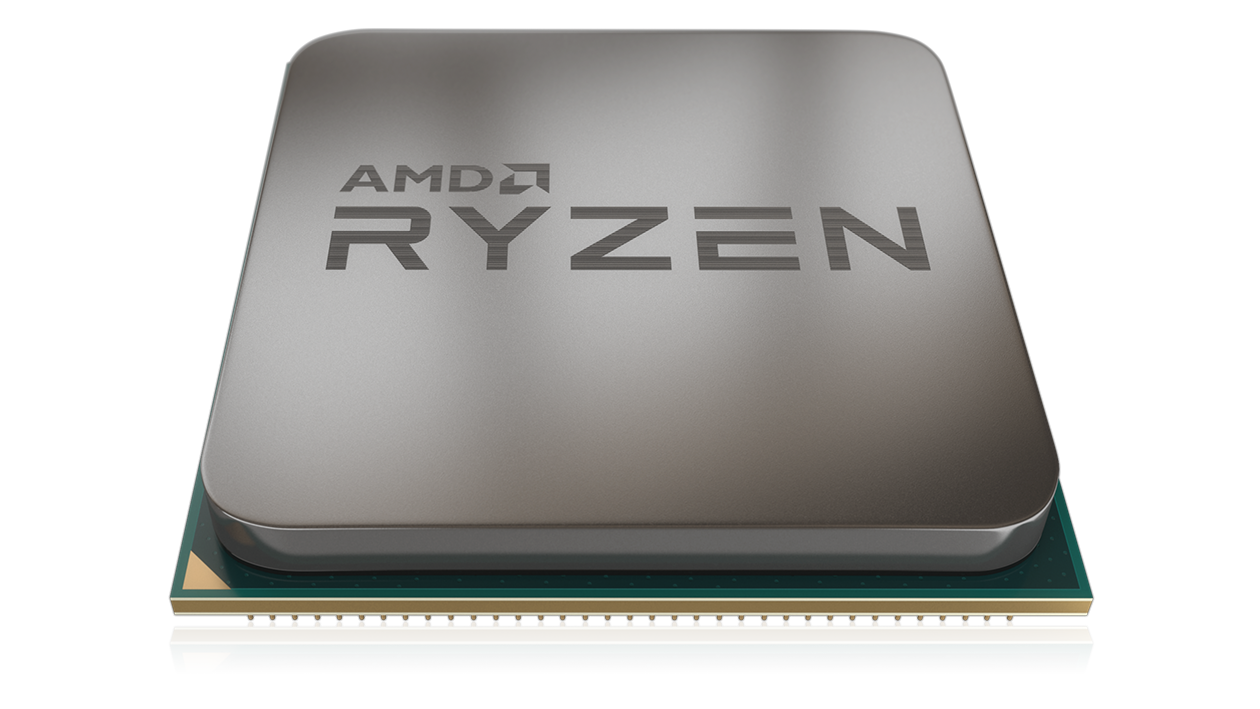
\includegraphics[scale=0.08]{data/cpu.png}};
            \node[] (image) at (0,4)
            {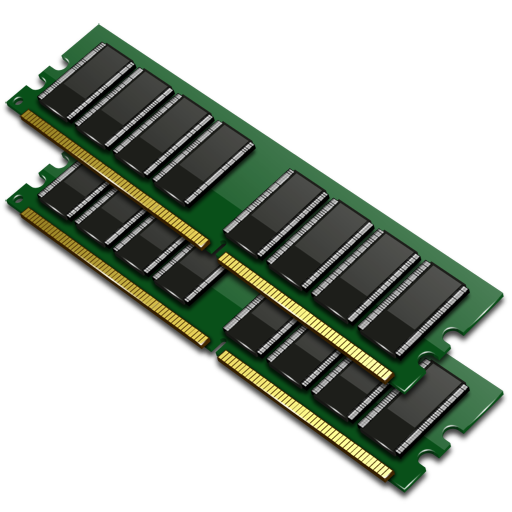
\includegraphics[scale=0.15]{data/ram.png}};
            \draw[<->,thick] (0,1.25) -- (0,2.75);
            \node[] at (-3,0) {CPU};
            \node[] at (-3,4) {RAM};
        \end{tikzpicture}
    \end{center}
\end{frame}

\begin{frame}[c, noframenumbering]{Memory Hierarchy}
    \begin{center}
        \begin{tikzpicture}
            \draw[fill=lightgray, rounded corners] (-4.5,1) rectangle (4.5,-3);
            \node[] (image) at (-4,-3)
            {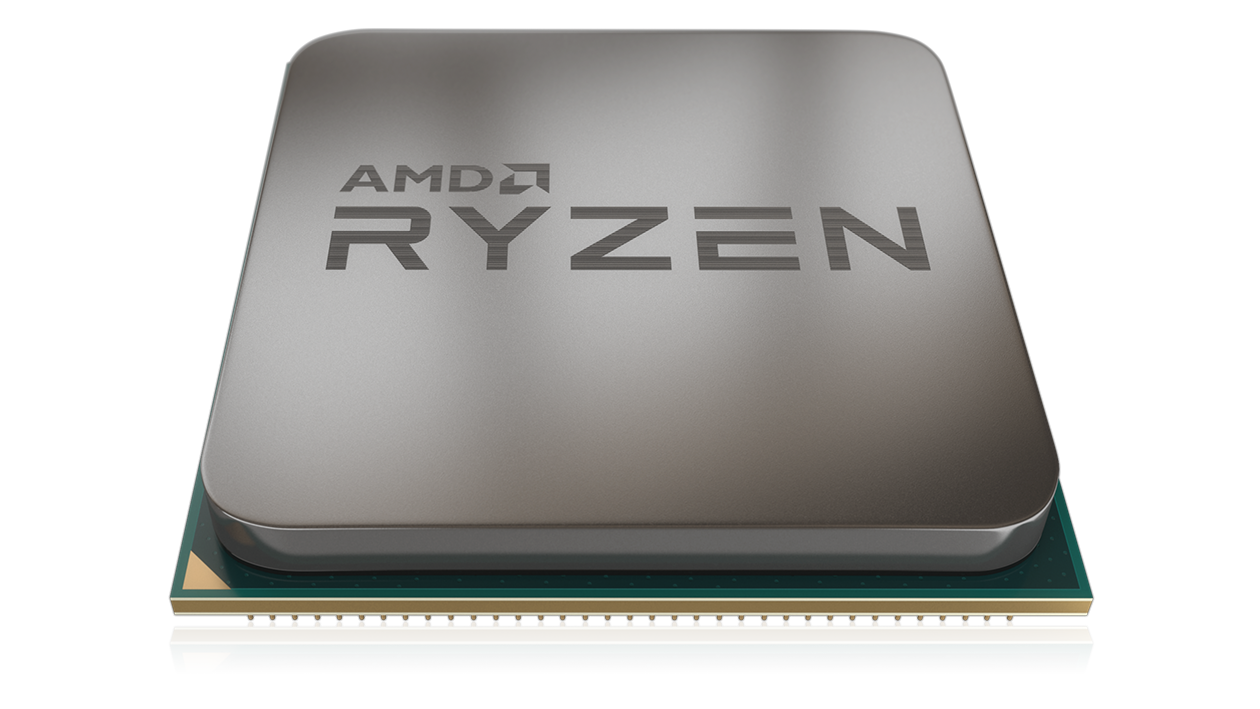
\includegraphics[scale=0.06]{data/cpu.png}};
            \node[] (image) at (0,3)
            {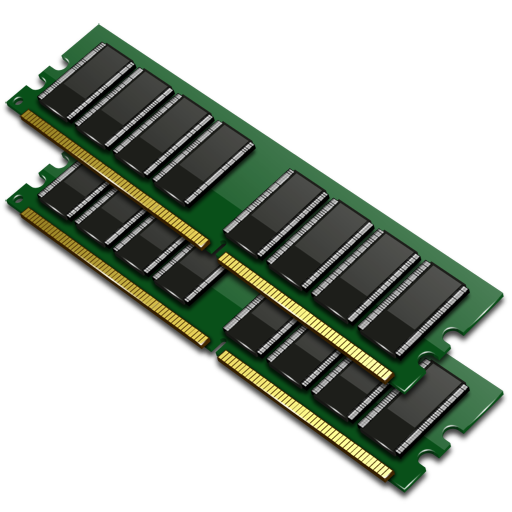
\includegraphics[scale=0.15]{data/ram.png}};
            \draw[<->,thick] (0,1.25) -- (0,1.75);
            \node[] at (-4,-2) {CPU};
            \node[] at (-4,3) {RAM};

            \draw[fill=white, rounded corners] (-3,0.5) rectangle (3,0) node
                [midway] {L3};
            \draw[fill=white, rounded corners] (-2,-0.5 + 0.5/3) rectangle
            (2,-1+0.5/3) node [midway] {L2};
            \draw[fill=white, rounded corners] (-1.5,-1.5 + 2*0.5/3) rectangle
            (1.5,-2+2*0.5/3) node [midway] {L1};
            \draw[fill=white, rounded corners] (-1,-2) rectangle (1,-2.5) node
                [midway] {Registers};

            \uncover<2-4>{
                \node[] at (-2,3) {\alert<2>{100ns}};
                \node[] at (-3.75,0.25) {\alert<2>{20ns}};
                \node[] at (-2.75,-1+0.5/3 + 0.25) {\alert<2>{5ns}};
                \node[] at (-1.5 - 0.75,-2+2*0.5/3 + 0.25) {\alert<2>{2ns}};
            }
            \uncover<3-4>{
                \node[] at (2,3) {\alert<3>{16GB}};
                \node[] at (3.75,0.25) {\alert<3>{15MB}};
                \node[] at (2.75,-1+0.5/3 + 0.25) {\alert<3>{256KB}};
                \node[] at (2.25,-2+2*0.5/3 + 0.25) {\alert<3>{32KB}};
                \node[] at (1.5,-2.25) {\alert<3>{16}};
            }

            \uncover<4>{
                \draw[fill=lightgray, rounded corners] (-4.5,2) rectangle
                (-0.5,1.25) node [midway] {\alert{64 bytes cache lines}};
            }
        \end{tikzpicture}
    \end{center}
\end{frame}

\begin{frame}[fragile,c]{Solution}
    \begin{itemize}
        \item Transpose $B$
              \pause
        \item But we’re not allowed to write to $B$
              \pause
        \item Instead, swap loop order
    \end{itemize}
    \pause
    \begin{exampleblock}{Python}
        \begin{minted}[
fontsize=\footnotesize,
linenos
]{python}
for i in range(M):
    for j in range(N):
        for k in range(K):
            C[i][j] += A[i][k] * B[k][j]
\end{minted}
    \end{exampleblock}
\end{frame}

\begin{frame}[fragile,c, noframenumbering]{Solution}
    \begin{itemize}
        \item Transpose $B$
        \item But we’re not allowed to write to $B$
        \item Instead, swap loop order
    \end{itemize}
    \begin{exampleblock}{Python}
        \begin{minted}[
fontsize=\footnotesize,
linenos
]{python}
for i in range(M):
    for k in range(K):
        for j in range(N):
            C[i][j] += A[i][k] * B[k][j]
\end{minted}
    \end{exampleblock}
\end{frame}

\begin{frame}{Illustration}
\end{frame}

\begin{frame}[c]{Performance Progression}

    \begin{figure}
        \centering
        \begin{tikzpicture}
            \begin{axis}[
                    width=0.9\textwidth,
                    height=0.8\textheight,
                    symbolic x coords={CPython,PyPy 3,C,C Transposed},
                    xtick=data,
                    axis x line=center,
                    axis y line=left,
                    enlargelimits=true,
                    enlarge x limits=0.25,
                    ylabel={GFLOPS},
                    nodes near coords,
                    nodes near coords style={font=\tiny},
                    every axis plot/.append style={
                            ybar,
                            bar width=20,
                            bar shift=0pt,
                            fill
                        }]
                \addplot[ybar,fill=blue,width=10] coordinates {
                        (CPython,0.004)
                        (PyPy 3,0.13)
                        (C,0.49)
                        (C Transposed, 1.95)
                    };
            \end{axis}
        \end{tikzpicture}
        \caption{i7-9750H CPU locked at 2 GHz using single precision floats}
        \label{fig:enter-label}
    \end{figure}
\end{frame}

\begin{frame}[fragile, c]{Single Instruction, Multiple Data (SIMD)}
    \pause
    \begin{exampleblock}{C}
        \begin{minted}[
fontsize=\footnotesize,
linenos
]{C}
int c = a + b;
\end{minted}
    \end{exampleblock}
    \pause
    \vfill
    \begin{exampleblock}{ASM}
        \begin{minted}[
fontsize=\footnotesize,
linenos
]{gas}
mov    a,%r1
mov    b,%r2
add    %r1,%r2
mov    %r2,c
\end{minted}
    \end{exampleblock}
\end{frame}

\begin{frame}[fragile, c]{Single Instruction, Multiple Data (SIMD)}
    \begin{center}
        \begin{tikzpicture}
            \draw[fill=white, rounded corners] (0,0) rectangle (7,1);
            \draw[fill=white, rounded corners] (0,2) rectangle (7,3);
            \node[] at (-1,0.5) {r2};
            \node[] at (-1,2.5) {r1};
            \draw [decorate,decoration={brace, amplitude=5pt, raise=2pt}] (0,3)
            -- (7,3) node[midway, yshift=0.5cm]{64-bit};

            \only<2>{
                \draw (3.5,0) -- (3.5,1);
                \draw (3.5,2) -- (3.5,3);

                \node[] at (5.25, 0.5) {32-bit};
                \node[] at (5.25, 2.5) {32-bit};

                \draw (5.25,1) -- (5.25,1.23);
                \draw (5.25,1.77) -- (5.25,2);
                \draw (5.25,1.5) circle (7.5pt) node{$+$};
            }
            \only<3>{
                \draw (3.5,0) -- (3.5,1);
                \draw (3.5,2) -- (3.5,3);

                \node[] at (5.25, 0.5) {32-bit};
                \node[] at (5.25, 2.5) {32-bit};

                \draw (5.25,1) -- (5.25,1.23);
                \draw (5.25,1.77) -- (5.25,2);
                \draw (5.25,1.5) circle (7.5pt) node{$+$};

                \node[] at (1.75, 0.5) {32-bit};
                \node[] at (1.75, 2.5) {32-bit};

                \draw (1.75,1) -- (1.75,1.23);
                \draw (1.75,1.77) -- (1.75,2);
                \draw (1.75,1.5) circle (7.5pt) node{$+$};
            }
            \only<4> {
                \foreach \i in {1.75,3.5,5.25} {
                        \draw (\i,0) -- (\i,1);
                        \draw (\i,2) -- (\i,3);
                    }
                \foreach \i in {0.875, 2.625, 4.375, 6.125} {
                        \node[] at (\i, 0.5) {16-bit};
                        \node[] at (\i, 2.5) {16-bit};

                        \draw (\i,1) -- (\i,1.23);
                        \draw (\i,1.77) -- (\i,2);
                        \draw (\i,1.5) circle (7.5pt) node{$+$};
                    }
            }
        \end{tikzpicture}
    \end{center}
\end{frame}

\begin{frame}[fragile,c]{Single Instruction, Multiple Data (SIMD)}
    \pause
    \begin{exampleblock}{C}
        \begin{minted}[
fontsize=\footnotesize,
linenos
]{C}
c[0] = a[0] + b[0];
c[1] = a[1] + b[1];
c[2] = a[2] + b[2];
c[3] = a[3] + b[3];
\end{minted}
    \end{exampleblock}
    \pause
    \vfill
    \begin{exampleblock}{ASM}
        \begin{minted}[
fontsize=\footnotesize,
linenos
]{gas}
movq    a,%r1
movq    b,%r2
paddw   %r1,%r2
movq    %r2,c
\end{minted}
    \end{exampleblock}
\end{frame}

\begin{frame}[c]{Single Instruction, Multiple Data (SIMD)}
    \begin{itemize}
        \item Intel MMX in 1997, lower precision integers in 64-bit registers
              \pause
        \item AMD 3DNow in 1998, supported single-precision floating-point
              values
              \pause
        \item Streaming SIMD extensions (SSE) \\ Intel in 1999 \\ \alert{Added
                  128-bit registers} \\ SSE2 to SSE4.2 (2000-2008)
              \pause
        \item Advanced Vector Extensions (AVX) \\ Intel in 2011 \\ \alert{Added
                  256-bit registers} \\ AVX2 in 2013
              \pause
        \item AVX-512 \\ Intel in 2017 \\ \alert{Added 512-bit registers}
    \end{itemize}
\end{frame}

\begin{frame}[c]{Performance Progression}

    \begin{figure}
        \centering
        \begin{tikzpicture}
            \begin{axis}[
                    width=0.9\textwidth,
                    height=0.75\textheight,
                    symbolic x coords={CPython,PyPy 3,C,C Transposed, C Vectorized},
                    xtick=data,
                    axis x line=center,
                    axis y line=left,
                    enlargelimits=true,
                    enlarge x limits=0.25,
                    x tick label style={font=\tiny,rotate=45, anchor=east},
                    ylabel={GFLOPS},
                    nodes near coords,
                    nodes near coords style={font=\tiny},
                    every axis plot/.append style={
                            ybar,
                            bar width=20,
                            bar shift=0pt,
                            fill
                        }]
                \addplot[ybar,fill=blue,width=10] coordinates {
                        (CPython,0.004)
                        (PyPy 3,0.13)
                        (C,0.49)
                        (C Transposed, 1.95)
                        (C Vectorized, 7.81)
                    };
            \end{axis}
        \end{tikzpicture}
        \caption{i7-9750H CPU locked at 2 GHz using single precision floats}
        \label{fig:enter-label}
    \end{figure}
\end{frame}

\begin{frame}[c]{What is the theoretical limit?}
    \pause
    \begin{figure}
        \centering
        \includegraphics[scale=0.25]{data/Screenshot from 2023-10-11
            22-25-17.png}
    \end{figure}
\end{frame}

\begin{frame}[c]{What is the theoretical limit?}
    \begin{itemize}
        \item Fused-multiply-add (FMA), computes $A * B + C$ in one instruction
    \end{itemize}
    \pause
    \begin{center}
        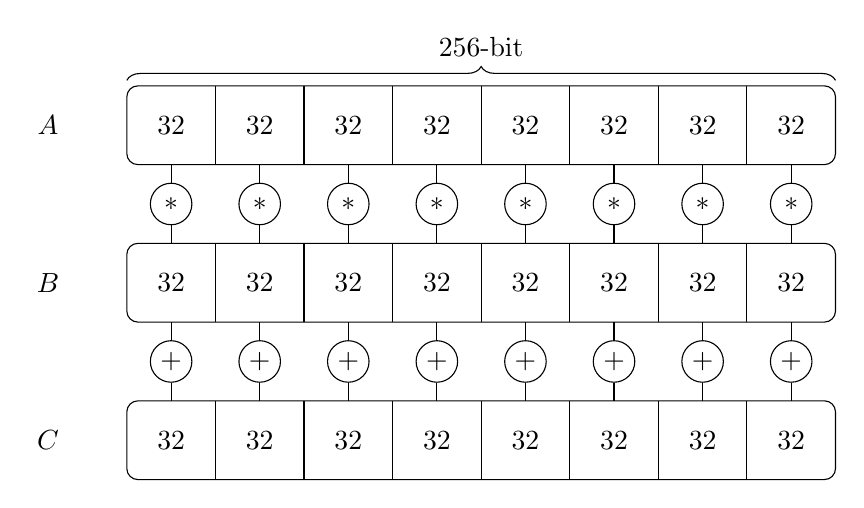
\begin{tikzpicture}
            \draw[fill=white, rounded corners] (0,0) rectangle (9,1);
            \draw[fill=white, rounded corners] (0,2) rectangle (9,3);
            \draw[fill=white, rounded corners] (0,4) rectangle (9,5);
            \node[] at (-1,0.5) {$C$};
            \node[] at (-1,2.5) {$B$};
            \node[] at (-1,4.5) {$A$};
            \draw [decorate,decoration={brace, amplitude=5pt, raise=2pt}] (0,5)
            -- (9,5) node[midway, yshift=0.5cm]{256-bit};

            \foreach \i in
                {1.125,2*1.125,3*1.125,4*1.125,5*1.125,6*1.125,7.875} {
                    \draw (\i,0) -- (\i,1);
                    \draw (\i,2) -- (\i,3);
                    \draw (\i,4) -- (\i,5);
                }
            \foreach \i in {0,1,2,3,4,5,6,7} {
                    \node[] at (0.5625 + \i * 1.125, 0.5) {32};
                    \node[] at (0.5625 + \i * 1.125, 2.5) {32};
                    \node[] at (0.5625 + \i * 1.125, 4.5) {32};

                    \draw (0.5625 + \i * 1.125,3) -- (0.5625 + \i *
                    1.125,3.23);
                    \draw (0.5625 + \i * 1.125,3.77) -- (0.5625 + \i *
                    1.125,4);
                    \draw (0.5625 + \i * 1.125,3.5) circle (7.5pt) node{$*$};

                    \draw (0.5625 + \i * 1.125,1) -- (0.5625 + \i *
                    1.125,1.23);
                    \draw (0.5625 + \i * 1.125,1.77) -- (0.5625 + \i *
                    1.125,2);
                    \draw (0.5625 + \i * 1.125,1.5) circle (7.5pt) node{$+$};
                }

        \end{tikzpicture}
    \end{center}
\end{frame}

\begin{frame}[fragile, c]{FMA benchmark}
    \pause
    \begin{exampleblock}{C}
        \begin{minted}[
fontsize=\footnotesize,
linenos
]{C}
v8sf A[N / 8], B[N / 8], C[N / 8];

for (int i = 0; i < N / 8; i++) {
	C[i] += A[i] * B[i];
}
\end{minted}
    \end{exampleblock}
    \pause
    \begin{exampleblock}{ASM}
        \begin{minted}[
fontsize=\footnotesize,
linenos
]{gas}
vmovps    A,%ymm0
vmovps    B,%ymm1
vmovps    C,%ymm2
vfmaddps  %ymm0,%ymm1,%ymm2
vmovps    %ymm2,C
\end{minted}
    \end{exampleblock}
\end{frame}

\begin{frame}{FMA benchmark}
    \begin{figure}
        \centering
        \begin{tikzpicture}
            \begin{semilogxaxis}[
                    width=\textwidth*0.9,
                    height=\axisdefaultheight*1,
                    line width=1pt,
                    legend cell align={left},
                    legend style={font=\footnotesize},
                    cycle list name=exotic,
                    xlabel={$N$},
                    xmode=log,
                    log basis x={2},
                    minor x tick num=4,
                    xmin=256,
                    xmax=62914560,
                    ylabel={GFLOPS},
                    ymin=0,
                    ymax=66,
                    ytick={0,16,32,48,64},
                    ymajorgrids=true
                ]

                \addplot+ [mark=none] table
                    {data/FMA_0.dat};

                \addplot +[mark=none, gray, dashed] coordinates {(8000, 1) (8000,
                        63)};
                \addplot +[mark=none, gray, dashed] coordinates {(64000, 1) (64000,
                        63)};
                \addplot +[mark=none, gray, dashed] coordinates {(3000000, 1)
                        (3000000, 63)};

                \legend{C[i] += A[i] $*$ B[i]};
            \end{semilogxaxis}
        \end{tikzpicture}
    \end{figure}
\end{frame}

\begin{frame}[fragile, c]{FMA benchmark, simplify}
    \pause
    \begin{exampleblock}{C}
        \begin{minted}[
fontsize=\footnotesize,
linenos
]{C}
v8sf A[N / 8], B[N / 8], C = {};

for (int i = 0; i < N / 8; i++) {
	C += A[i] * B[i];
}
\end{minted}
    \end{exampleblock}
    \pause
    \begin{exampleblock}{ASM}
        \begin{minted}[
fontsize=\footnotesize,
linenos
]{gas}
vmovps    A,%ymm0
vmovps    B,%ymm1
vfmaddps  %ymm0,%ymm1,%ymm2
\end{minted}
    \end{exampleblock}
\end{frame}

\begin{frame}{FMA benchmark, simplified}
    \begin{figure}
        \centering
        \begin{tikzpicture}
            \begin{semilogxaxis}[
                    width=\textwidth*0.9,
                    height=\axisdefaultheight*1,
                    line width=1pt,
                    legend cell align={left},
                    legend style={font=\footnotesize},
                    cycle list name=exotic,
                    xlabel={$N$},
                    xmode=log,
                    log basis x={2},
                    minor x tick num=4,
                    xmin=256,
                    xmax=62914560,
                    ylabel={GFLOPS},
                    ymin=0,
                    ymax=66,
                    ytick={0,16,32,48,64},
                    ymajorgrids=true
                ]

                \addplot+ [mark=none] table
                    {data/FMA_0.dat};
                \addplot+ [mark=none] table
                    {data/FMA_1.dat};

                \addplot +[mark=none, gray, dashed] coordinates {(8000, 1) (8000,
                        63)};
                \addplot +[mark=none, gray, dashed] coordinates {(64000, 1) (64000,
                        63)};
                \addplot +[mark=none, gray, dashed] coordinates {(3000000, 1)
                        (3000000, 63)};

                \legend{C[i] += A[i] $*$ B[i],
                    C += A[i] $*$ B[i]};
            \end{semilogxaxis}
        \end{tikzpicture}
    \end{figure}
\end{frame}

\begin{frame}[fragile, c]{FMA benchmark, simplified}
    \pause
    \begin{exampleblock}{C}
        \begin{minted}[
fontsize=\footnotesize,
linenos
]{C}
v8sf A[N / 8], B[N / 8], C1 = {}, C2 = {};

for (int i = 0; i < N / 8; i += 2) {
	C1 += A[i] * B[i];
	C2 += A[i + 1] * B[i + 1];
}

C1 += C2;
\end{minted}
    \end{exampleblock}
\end{frame}

\begin{frame}{FMA benchmark, simplified}
    \begin{figure}
        \centering
        \begin{tikzpicture}
            \begin{semilogxaxis}[
                    width=\textwidth*0.9,
                    height=\axisdefaultheight*1,
                    line width=1pt,
                    legend cell align={left},
                    legend style={font=\footnotesize},
                    cycle list name=exotic,
                    xlabel={$N$},
                    xmode=log,
                    log basis x={2},
                    minor x tick num=4,
                    xmin=256,
                    xmax=62914560,
                    ylabel={GFLOPS},
                    ymin=0,
                    ymax=66,
                    ytick={0,16,32,48,64},
                    ymajorgrids=true
                ]

                \addplot+ [mark=none] table
                    {data/FMA_0.dat};
                \addplot+ [mark=none] table
                    {data/FMA_2.dat};

                \addplot +[mark=none, gray, dashed] coordinates {(8000, 1) (8000,
                        63)};
                \addplot +[mark=none, gray, dashed] coordinates {(64000, 1) (64000,
                        63)};
                \addplot +[mark=none, gray, dashed] coordinates {(3000000, 1)
                        (3000000, 63)};

                \legend{C[i] += A[i] $*$ B[i],
                    C += A[i] $*$ B[i]};
            \end{semilogxaxis}
        \end{tikzpicture}
    \end{figure}
\end{frame}

\begin{frame}[fragile, c]{FMA benchmark, what's the problem?}
    \pause
    \begin{exampleblock}{ASM}
        \begin{minted}[
fontsize=\footnotesize,
linenos
]{gas}
vmovps    A,%ymm0
vmovps    B,%ymm1
vfmaddps  %ymm0,%ymm1,%ymm2
\end{minted}
    \end{exampleblock}

    \pause

    \begin{itemize}
        \item We can do 2 FMAs per cycle
              \pause
        \item But.. We're also limited to 2 moves per cycle
    \end{itemize}

\end{frame}

\begin{frame}[fragile, c]{FMA benchmark, simplify further}
    \pause
    \begin{exampleblock}{C}
        \begin{minted}[
fontsize=\footnotesize,
linenos
]{C}
v8sf A = {}, B[N / 8], C1 = {}, C2 = {};

for (int i = 0; i < N / 8; i + 1) {
    C1 += A * B[i];
    C2 += A * B[i + 1];
}

C1 += C2;
\end{minted}
    \end{exampleblock}
\end{frame}

\begin{frame}{FMA benchmark}
    \begin{figure}
        \centering
        \begin{tikzpicture}
            \begin{semilogxaxis}[
                    width=\textwidth*0.9,
                    height=\axisdefaultheight*1,
                    line width=1pt,
                    legend cell align={left},
                    legend style={font=\footnotesize},
                    cycle list name=exotic,
                    xlabel={$N$},
                    xmode=log,
                    log basis x={2},
                    minor x tick num=4,
                    xmin=256,
                    xmax=62914560,
                    ylabel={GFLOPS},
                    ymin=0,
                    ymax=66,
                    ytick={0,16,32,48,64},
                    ymajorgrids=true
                ]

                \addplot+ [mark=none] table
                    {data/FMA_0.dat};
                \addplot+ [mark=none] table
                    {data/FMA_2.dat};
                \addplot+ [mark=none] table
                    {data/FMA_3.dat};

                \addplot +[mark=none, gray, dashed] coordinates {(8000, 1) (8000,
                        63)};
                \addplot +[mark=none, gray, dashed] coordinates {(64000, 1) (64000,
                        63)};
                \addplot +[mark=none, gray, dashed] coordinates {(3000000, 1)
                        (3000000, 63)};

                \legend{C[i] += A[i] $*$ B[i],
                    C += A[i] $*$ B[i],
                    C += A $*$ B[i]};
            \end{semilogxaxis}
        \end{tikzpicture}
    \end{figure}
\end{frame}

\begin{frame}[noframenumbering]{FMA benchmark}
    \begin{figure}
        \centering
        \begin{tikzpicture}
            \begin{semilogxaxis}[
                    width=\textwidth*0.9,
                    height=\axisdefaultheight*1,
                    line width=1pt,
                    legend cell align={left},
                    legend style={font=\footnotesize},
                    cycle list name=exotic,
                    xlabel={$N$},
                    xmode=log,
                    log basis x={2},
                    minor x tick num=4,
                    xmin=256,
                    xmax=62914560,
                    ylabel={GFLOPS},
                    ymin=0,
                    ymax=66,
                    ytick={0,16,32,48,64},
                    ymajorgrids=true
                ]

                \addplot+ [mark=none] table
                    {data/FMA_0.dat};
                \addplot+ [mark=none] table
                    {data/FMA_2.dat};
                \addplot+ [mark=none] table
                    {data/FMA_3.dat};
                \addplot+ [mark=none] table
                    {data/FMA_4.dat};

                \addplot +[mark=none, gray, dashed] coordinates {(8000, 1) (8000,
                        63)};
                \addplot +[mark=none, gray, dashed] coordinates {(64000, 1) (64000,
                        63)};
                \addplot +[mark=none, gray, dashed] coordinates {(3000000, 1)
                        (3000000, 63)};

                \legend{C[i] += A[i] $*$ B[i],
                    C += A[i] $*$ B[i],
                    C += A $*$ B[i],
                    C += A $*$ B[i] (x2)};
            \end{semilogxaxis}
        \end{tikzpicture}
    \end{figure}
\end{frame}

\begin{frame}{Cache blocking example}
\end{frame}

\begin{frame}[c]{The OpenBLAS Implementation}
    \begin{itemize}
        \item Needs aligned memory for vector instructions
        \item Don’t want to allocate new memory for the entire matrix
        \item Instead, allocate L2 sized array for A, and L1 sized array for B
        \item Place the data in buffers based on how it will be accessed

    \end{itemize}
\end{frame}

\begin{frame}[fragile, c]{OpenBLAS Macro View}
    \begin{center}
        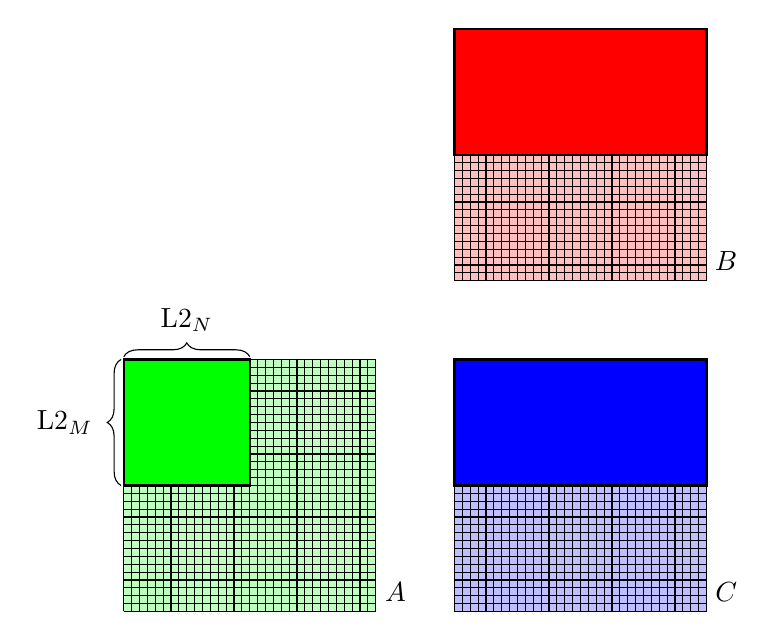
\begin{tikzpicture}
            \draw (3.45,0.25) node{$A$};
            \fill[green, opacity=0.25] (0,0) rectangle ++(3.2,3.2);
            \draw[step=0.1cm,black] (0,0) grid ++(3.2,3.2);

            \draw (7.65,0.25) node{$C$};
            \fill[blue, opacity=0.25] (4.2,0) rectangle ++(3.2,3.2);
            \draw[step=0.1cm,black] (4.2-0.001,0-0.001) grid
            ++(3.2+0.003,3.2+0.003);

            \draw (7.65,4.45) node{$B$};
            \fill[red, opacity=0.25] (4.2,4.2) rectangle ++(3.2,3.2);
            \draw[step=0.1cm,black] (4.2-0.001,4.2-0.001) grid
            ++(3.2+0.003,3.2+0.003);

            \uncover<2-4> {
                \fill[green] (0,1.6) rectangle ++(1.6,1.6);
                \draw[black, thick] (0,1.6) rectangle ++(1.6,1.6);
            }
            \uncover<3-4> {
                \draw [decorate,decoration={brace, amplitude=5pt, raise=1pt}]
                (0,3.2) -- (1.6,3.2) node[midway, yshift=0.5cm]{L$2_N$};
                \draw [decorate,decoration={brace, amplitude=5pt, raise=1pt}]
                (0,1.6) -- (0,3.2) node[midway, xshift=-0.75cm]{L$2_M$};
            }
            \uncover<4> {
                \fill[blue] (4.2,1.6) rectangle ++(3.2,1.6);
                \draw[black, thick] (4.2,1.6) rectangle ++(3.2,1.6);

                \fill[red] (4.2,4.2+1.6) rectangle ++(3.2,1.6);
                \draw[black, thick] (4.2,4.2+1.6) rectangle ++(3.2,1.6);
            }
        \end{tikzpicture}
    \end{center}
\end{frame}

\hidelogo
\begin{frame}[fragile, c, noframenumbering]{OpenBLAS Macro View}
    \begin{center}
        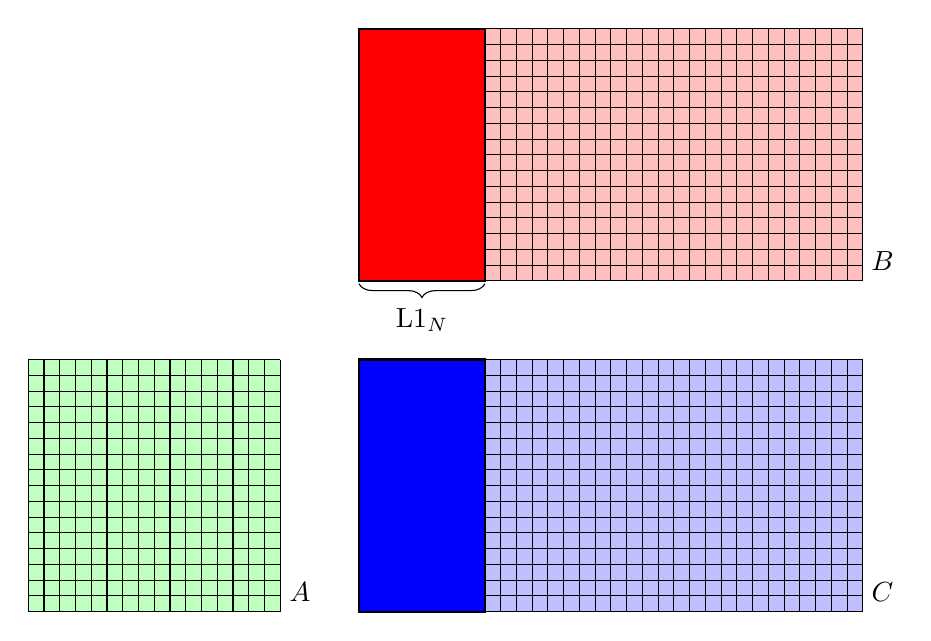
\begin{tikzpicture}
            \draw (3.45,0.25) node{$A$};
            \fill[green, opacity=0.25] (0,0) rectangle ++(3.2,3.2);
            \draw[step=0.2cm,black] (0,0) grid ++(3.2,3.2);

            \draw (7.65+3.2,0.25) node{$C$};
            \fill[blue, opacity=0.25] (4.2,0) rectangle ++(6.4,3.2);
            \draw[step=0.2cm,black] (4.2-0.001,0-0.001) grid
            ++(6.4+0.003,3.2+0.003);

            \draw (7.65+3.2,4.45) node{$B$};
            \fill[red, opacity=0.25] (4.2,4.2) rectangle ++(6.4,3.2);
            \draw[step=0.2cm,black] (4.2-0.001,4.2-0.001) grid
            ++(6.4+0.003,3.2+0.003);

            \uncover<2-3> {
                \fill[red] (4.2,4.2) rectangle ++(1.6,3.2);
                \draw[black, thick] (4.2-0.001,4.2-0.001) rectangle
                ++(1.6+0.003,3.2+0.003);
                \draw [decorate,decoration={brace, amplitude=5pt, raise=1pt}]
                (4.2+1.6,4.2) -- (4.2,4.2) node[midway, yshift=-0.5cm]{L$1_N$};
            }
            \uncover<3> {
                \fill[blue] (4.2,0) rectangle ++(1.6,3.2);
                \draw[black, thick] (4.2-0.001,0-0.001) rectangle
                ++(1.6+0.003,3.2+0.003);
            }
        \end{tikzpicture}
    \end{center}
\end{frame}

\showlogo

\begin{frame}[c, noframenumbering]{OpenBLAS Macro View}
    \begin{center}
        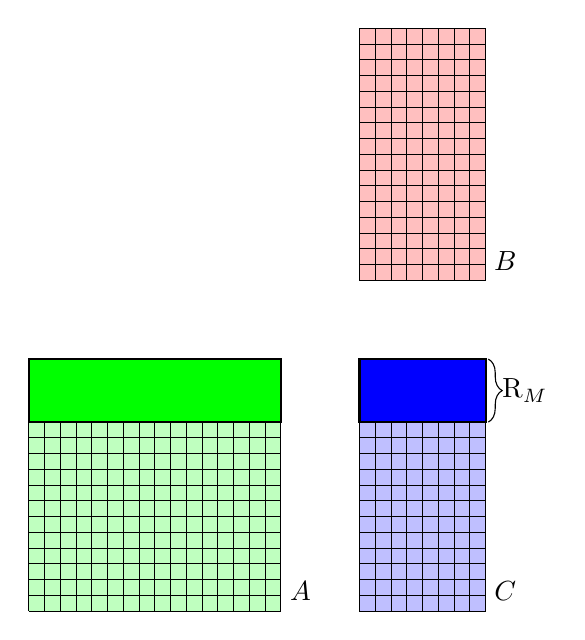
\begin{tikzpicture}
            \draw (3.45,0.25) node{$A$};
            \fill[green, opacity=0.25] (0,0) rectangle ++(3.2,3.2);
            \draw[step=0.2cm,black] (0,0) grid ++(3.2,3.2);

            \draw (6.05,0.25) node{$C$};
            \fill[blue, opacity=0.25] (4.2,0) rectangle ++(1.6,3.2);
            \draw[step=0.2cm,black] (4.2-0.001,0-0.001) grid
            ++(1.6+0.003,3.2+0.003);

            \draw (6.05,4.45) node{$B$};
            \fill[red, opacity=0.25] (4.2,4.2) rectangle ++(1.6,3.2);
            \draw[step=0.2cm,black] (4.2-0.001,4.2-0.001) grid
            ++(1.6+0.003,3.2+0.003);

            \uncover<2-3> {
                \fill[blue] (4.2,0.8*3) rectangle ++(1.6,0.8);
                \draw[black, thick] (4.2-0.001,0.8*3-0.001) rectangle
                ++(1.6+0.003,0.8+0.003);
                \draw [decorate,decoration={brace, amplitude=5pt, raise=1pt}]
                (4.2+1.6,3.2) -- (4.2+1.6,3.2-0.8) node[midway, xshift=0.5cm]{R$_M$};
            }
            \uncover<3> {
                \fill[green] (0,3.2-0.8) rectangle ++(3.2,0.8);
                \draw[black, thick] (0-0.001,3.2-0.8-0.001) rectangle
                ++(3.2+0.003,0.8+0.003);
            }
        \end{tikzpicture}
    \end{center}
\end{frame}

\begin{frame}[c, noframenumbering]{OpenBLAS Macro View}
    \begin{center}
        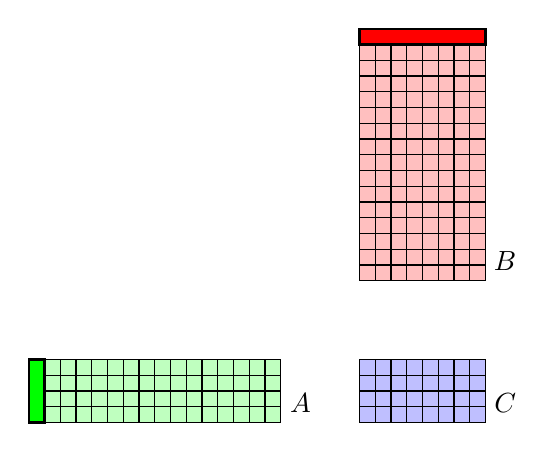
\begin{tikzpicture}
            \draw (3.45,0.25) node{$A$};
            \fill[green, opacity=0.25] (0,0) rectangle ++(3.2,0.8);
            \draw[step=0.2cm,black] (0,0) grid ++(3.2,0.8);

            \draw (6.05,0.25) node{$C$};
            \fill[blue, opacity=0.25] (4.2,0) rectangle ++(1.6,0.8);
            \draw[step=0.2cm,black] (4.2-0.001,0-0.001) grid
            ++(1.6+0.003,0.8+0.003);

            \draw (6.05,2.05) node{$B$};
            \fill[red, opacity=0.25] (4.2,1.8) rectangle ++(1.6,3.2);
            \draw[step=0.2cm,black] (4.2-0.001,1.8-0.001) grid
            ++(1.6+0.003,3.2+0.003);

            \uncover<2> {
                \fill[green] (0,0) rectangle ++(0.2,0.8);
                \draw[black, thick] (0,0) rectangle ++(0.2,0.8);

                \fill[red] (4.2,5-0.2) rectangle ++(1.6,0.2);
                \draw[black, thick] (4.2,5-0.2) rectangle ++(1.6,0.2);
            }
        \end{tikzpicture}
    \end{center}
\end{frame}
\section{References}

\begin{frame}[c]{OpenBLAS Micro View}
    \begin{center}
        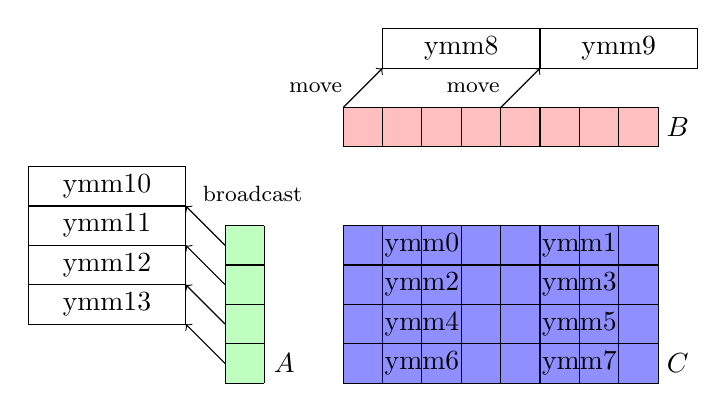
\begin{tikzpicture}
            \draw (0.75,0.25) node{$A$};
            \fill[green, opacity=0.25] (0,0) rectangle ++(0.5,2);
            \draw[step=0.5cm,black] (0,0) grid ++(0.5,2);

            \draw (5.75,0.25) node{$C$};
            \only<1> {
                \fill[blue, opacity=0.25] (1.5,0) rectangle ++(4,2);
                \draw[step=0.5cm,black] (1.5-0.001,0-0.001) grid
                ++(4+0.003,2+0.003);
            }

            \draw (5.75,3.25) node{$B$};
            \fill[red, opacity=0.25] (1.5,3) rectangle ++(4,0.5);
            \draw[step=0.5cm,black] (1.5-0.001,3-0.001) grid
            ++(4+0.003,0.5+0.003);

            \uncover<2-> {
                \fill[blue, opacity=0.25] (1.5,0) rectangle ++(4,2);
                \draw[black] (1.5,0) rectangle ++(4,2);
                \draw[black] (1.5,0.5) -- (5.5,0.5);
                \draw[black] (1.5,1) -- (5.5,1);
                \draw[black] (1.5,1.5) -- (5.5,1.5);
                \draw[black] (3.5,0) -- (3.5,2);

                \draw (2.5, 1.75) node{ymm0};
                \draw (4.5, 1.75) node{ymm1};
                \draw (2.5, 1.25) node{ymm2};
                \draw (4.5, 1.25) node{ymm3};
                \draw (2.5, 0.75) node{ymm4};
                \draw (4.5, 0.75) node{ymm5};
                \draw (2.5, 0.25) node{ymm6};
                \draw (4.5, 0.25) node{ymm7};
            }
            \uncover<3->{
                \draw[->] (1.5,3.5) -- (2,4) node[midway,
                    xshift=-0.6cm]{\footnotesize{move}};
                \draw[->] (3.5,3.5) -- (4,4) node[midway,
                    xshift=-0.6cm]{\footnotesize{move}};
                \draw[black] (2,4) rectangle ++(2,0.5);
                \draw (3,4.25) node{ymm8};
                \draw[black] (4,4) rectangle ++(2,0.5);
                \draw (5,4.25) node{ymm9};
            }
            \uncover<4->{
                \draw[->] (0,1.75) -- (-0.5,2.25) node[midway, xshift=0.6cm,
                    yshift=0.4cm]{\footnotesize{broadcast}};
                \draw[->] (0,1.25) -- (-0.5,1.75);
                \draw[->] (0,0.75) -- (-0.5,1.25);
                \draw[->] (0,0.25) -- (-0.5,0.75);

                \draw[black] (-2.5,2.25) rectangle ++(2,0.5);
                \draw (-1.5,2.5) node{ymm10};
                \draw[black] (-2.5,1.75) rectangle ++(2,0.5);
                \draw (-1.5,2) node{ymm11};
                \draw[black] (-2.5,1.25) rectangle ++(2,0.5);
                \draw (-1.5,1.5) node{ymm12};
                \draw[black] (-2.5,0.75) rectangle ++(2,0.5);
                \draw (-1.5,1) node{ymm13};
            }
        \end{tikzpicture}
        \uncover<5-> {
            \begin{itemize}
                \item 6 move operations
                \item 8 FMA operations
            \end{itemize}
        }
    \end{center}
\end{frame}

\begin{frame}[fragile, c]{OpenBLAS Micro View}
    \begin{exampleblock}{ASM}
        \begin{minted}[
fontsize=\footnotesize,
linenos
]{gas}
vmovaps       (%rdx),%ymm1
vmovaps       0x20(%rdx),%ymm0

vbroadcastss  (%rax),%ymm2
vfmadd231ps   %ymm2,%ymm1,%ymm12
vfmadd231ps   %ymm2,%ymm0,%ymm11

vbroadcastss  0x4ac(%rax),%ymm2
vfmadd231ps   %ymm2,%ymm1,%ymm10
vfmadd231ps   %ymm2,%ymm0,%ymm9

...
\end{minted}
    \end{exampleblock}
\end{frame}

\begin{frame}[c]{Performance Progression}

    \begin{figure}
        \centering
        \begin{tikzpicture}
            \begin{axis}[
                    width=0.9\textwidth,
                    height=0.75\textheight,
                    symbolic x coords={CPython,PyPy 3,C,C Transposed, C Vectorized, C Block +
                            FMA, OpenBLAS},
                    xtick=data,
                    axis x line=center,
                    axis y line=left,
                    enlargelimits=true,
                    enlarge x limits=0.25,
                    x tick label style={font=\tiny,rotate=45, anchor=east},
                    ymax=64,
                    ytick={0,16,32,48,64},
                    ylabel={GFLOPS},
                    nodes near coords,
                    nodes near coords style={font=\tiny},
                    every axis plot/.append style={
                            ybar,
                            bar width=20,
                            bar shift=0pt,
                            fill
                        }]
                \addplot[ybar,fill=blue,width=10] coordinates {
                        (CPython,0.004)
                        (PyPy 3,0.13)
                        (C,0.49)
                        (C Transposed, 1.95)
                        (C Vectorized, 7.81)
                        (C Block + FMA, 52.5)
                        (OpenBLAS, 60.25)
                    };
                \draw[dashed] (axis cs:CPython,64) -- node[above,font=\small]{Theoretical
                    Limit} ++(500,0);
            \end{axis}
        \end{tikzpicture}
        \caption{i7-9750H CPU locked at 2 GHz using single precision floats}
        \label{fig:enter-label}
    \end{figure}
\end{frame}

\begin{frame}[allowframebreaks]{References}
    \tiny
    \begin{thebibliography}{}
        \setbeamertemplate{bibliography item}[article]
        \bibitem{Goto}
        Goto, K. and Geijn, R.A.V.D.
        \newblock \enquote{2008. Anatomy of high-performance matrix
            multiplication.}
        \newblock \emph{ACM Transactions on Mathematical Software (TOMS),
            34(3), pp.1-25.}

        \setbeamertemplate{bibliography item}[book]
        \bibitem{Sergey}
        Sergey Slotin
        \newblock \enquote{Algorithms for Modern Hardware}
        \newblock \url{https://en.algorithmica.org/hpc/}

        \bibitem{Kusswurm}
        Kusswurm, D.
        \newblock \enquote{Modern Parallel Programming with C++ and Assembly
            Language: X86 SIMD Development Using AVX, AVX2, and AVX-512.}

        \setbeamertemplate{bibliography item}[triangle]

        \bibitem{Jukka}
        Jukka Suomela, cache-blocking-demo

        \setbeamertemplate{bibliography item}[online]
        \bibitem{Burghardt2023}
        Jochen Burghardt
        \newblock \enquote{Computational complexity of matrix multiplication.
            (2023, September 3). In Wikipedia.}.
        \newblock
        \url{https://en.wikipedia.org/wiki/Computational_complexity_of_matrix_multiplication}

        \setbeamertemplate{bibliography item}[article]

        \bibitem{Strassen}
        Strassen, V.
        \newblock \enquote{1969. Gaussian elimination is not optimal.}
        \newblock \emph{Numerische mathematik, 13(4), pp.354-356.}

        \bibitem{Williams}
        Williams, V.V., Xu, Y., Xu, Z. and Zhou, R.
        \newblock \enquote{2023. New bounds for matrix multiplication: from
            alpha to omega.}
        \newblock \emph{arXiv preprint arXiv:2307.07970.}

        \bibitem{Douglas}
        Douglas, C.C., Heroux, M., Slishman, G. and Smith, R.M.
        \newblock \enquote{1994. GEMMW: A portable level 3 BLAS Winograd
            variant of Strassen's matrix-matrix multiply algorithm.}
        \newblock \emph{Journal of Computational Physics, 110(1), pp.1-10.}

        \bibitem{Huss}
        Huss-Lederman, S., Jacobson, E.M., Tsao, A., Turnbull, T. and Johnson,
        J.R.
        \newblock \enquote{1996, November. Implementation of Strassen's
            algorithm for matrix multiplication.}
        \newblock \emph{In Proceedings of the 1996 ACM/IEEE Conference on
            Supercomputing (pp. 32-es).}

        \bibitem{Bjørstad}
        Bjørstad, P., Manne, F., Sørevik, T. and Vajteršic, M.
        \newblock \enquote{1992. Efficient matrix multiplication on SIMD
            computers.}
        \newblock \emph{SIAM Journal on Matrix Analysis and Applications,
            13(1), pp.386-401.}

        \bibitem{Huang}
        Huang, J., Smith, T.M., Henry, G.M. and Van De Geijn, R.A.
        \newblock \enquote{2016, November. Strassen's algorithm reloaded.}
        \newblock \emph{In SC'16: Proceedings of the International Conference
            for High Performance Computing, Networking, Storage and Analysis (pp. 690-701).
            IEEE.}

        \bibitem{Dalberto}
        D'alberto, P., Bodrato, M. and Nicolau, A.
        \newblock \enquote{2011. Exploiting parallelism in matrix-computation
            kernels for symmetric multiprocessor systems: Matrix-multiplication and
            matrix-addition algorithm optimizations by software pipelining and threads
            allocation.}
        \newblock \emph{ACM Transactions on Mathematical Software (TOMS),
            38(1), pp.1-30.}

        \setbeamertemplate{bibliography item}[online]

        \bibitem{FLOPS}
        \url{https://en.wikipedia.org/wiki/FLOPS}

    \end{thebibliography}
\end{frame}

\end{document}